\documentclass[main]{subfiles}


\title[Dynamic Approaches]{Dynamic Approaches}
\subtitle{Population Based Methods}
\author[André Biedenkapp]{André Biedenkapp}
\date{}

\titlebackground*{images/AutoML_LearningToLearn2}

%\institute{}
%\date{}

\begin{document}
	
	\maketitle
%-----------------------------------------------------------------------
%----------------------------------------------------------------------
%-----------------------------------------------------------------------
%----------------------------------------------------------------------
%-----------------------------------------------------------------------
%----------------------------------------------------------------------
%-----------------------------------------------------------------------
%----------------------------------------------------------------------
%-----------------------------------------------------------------------
%----------------------------------------------------------------------
\begin{frame}{Towards On-the-Fly Adaptation}
        \centering
        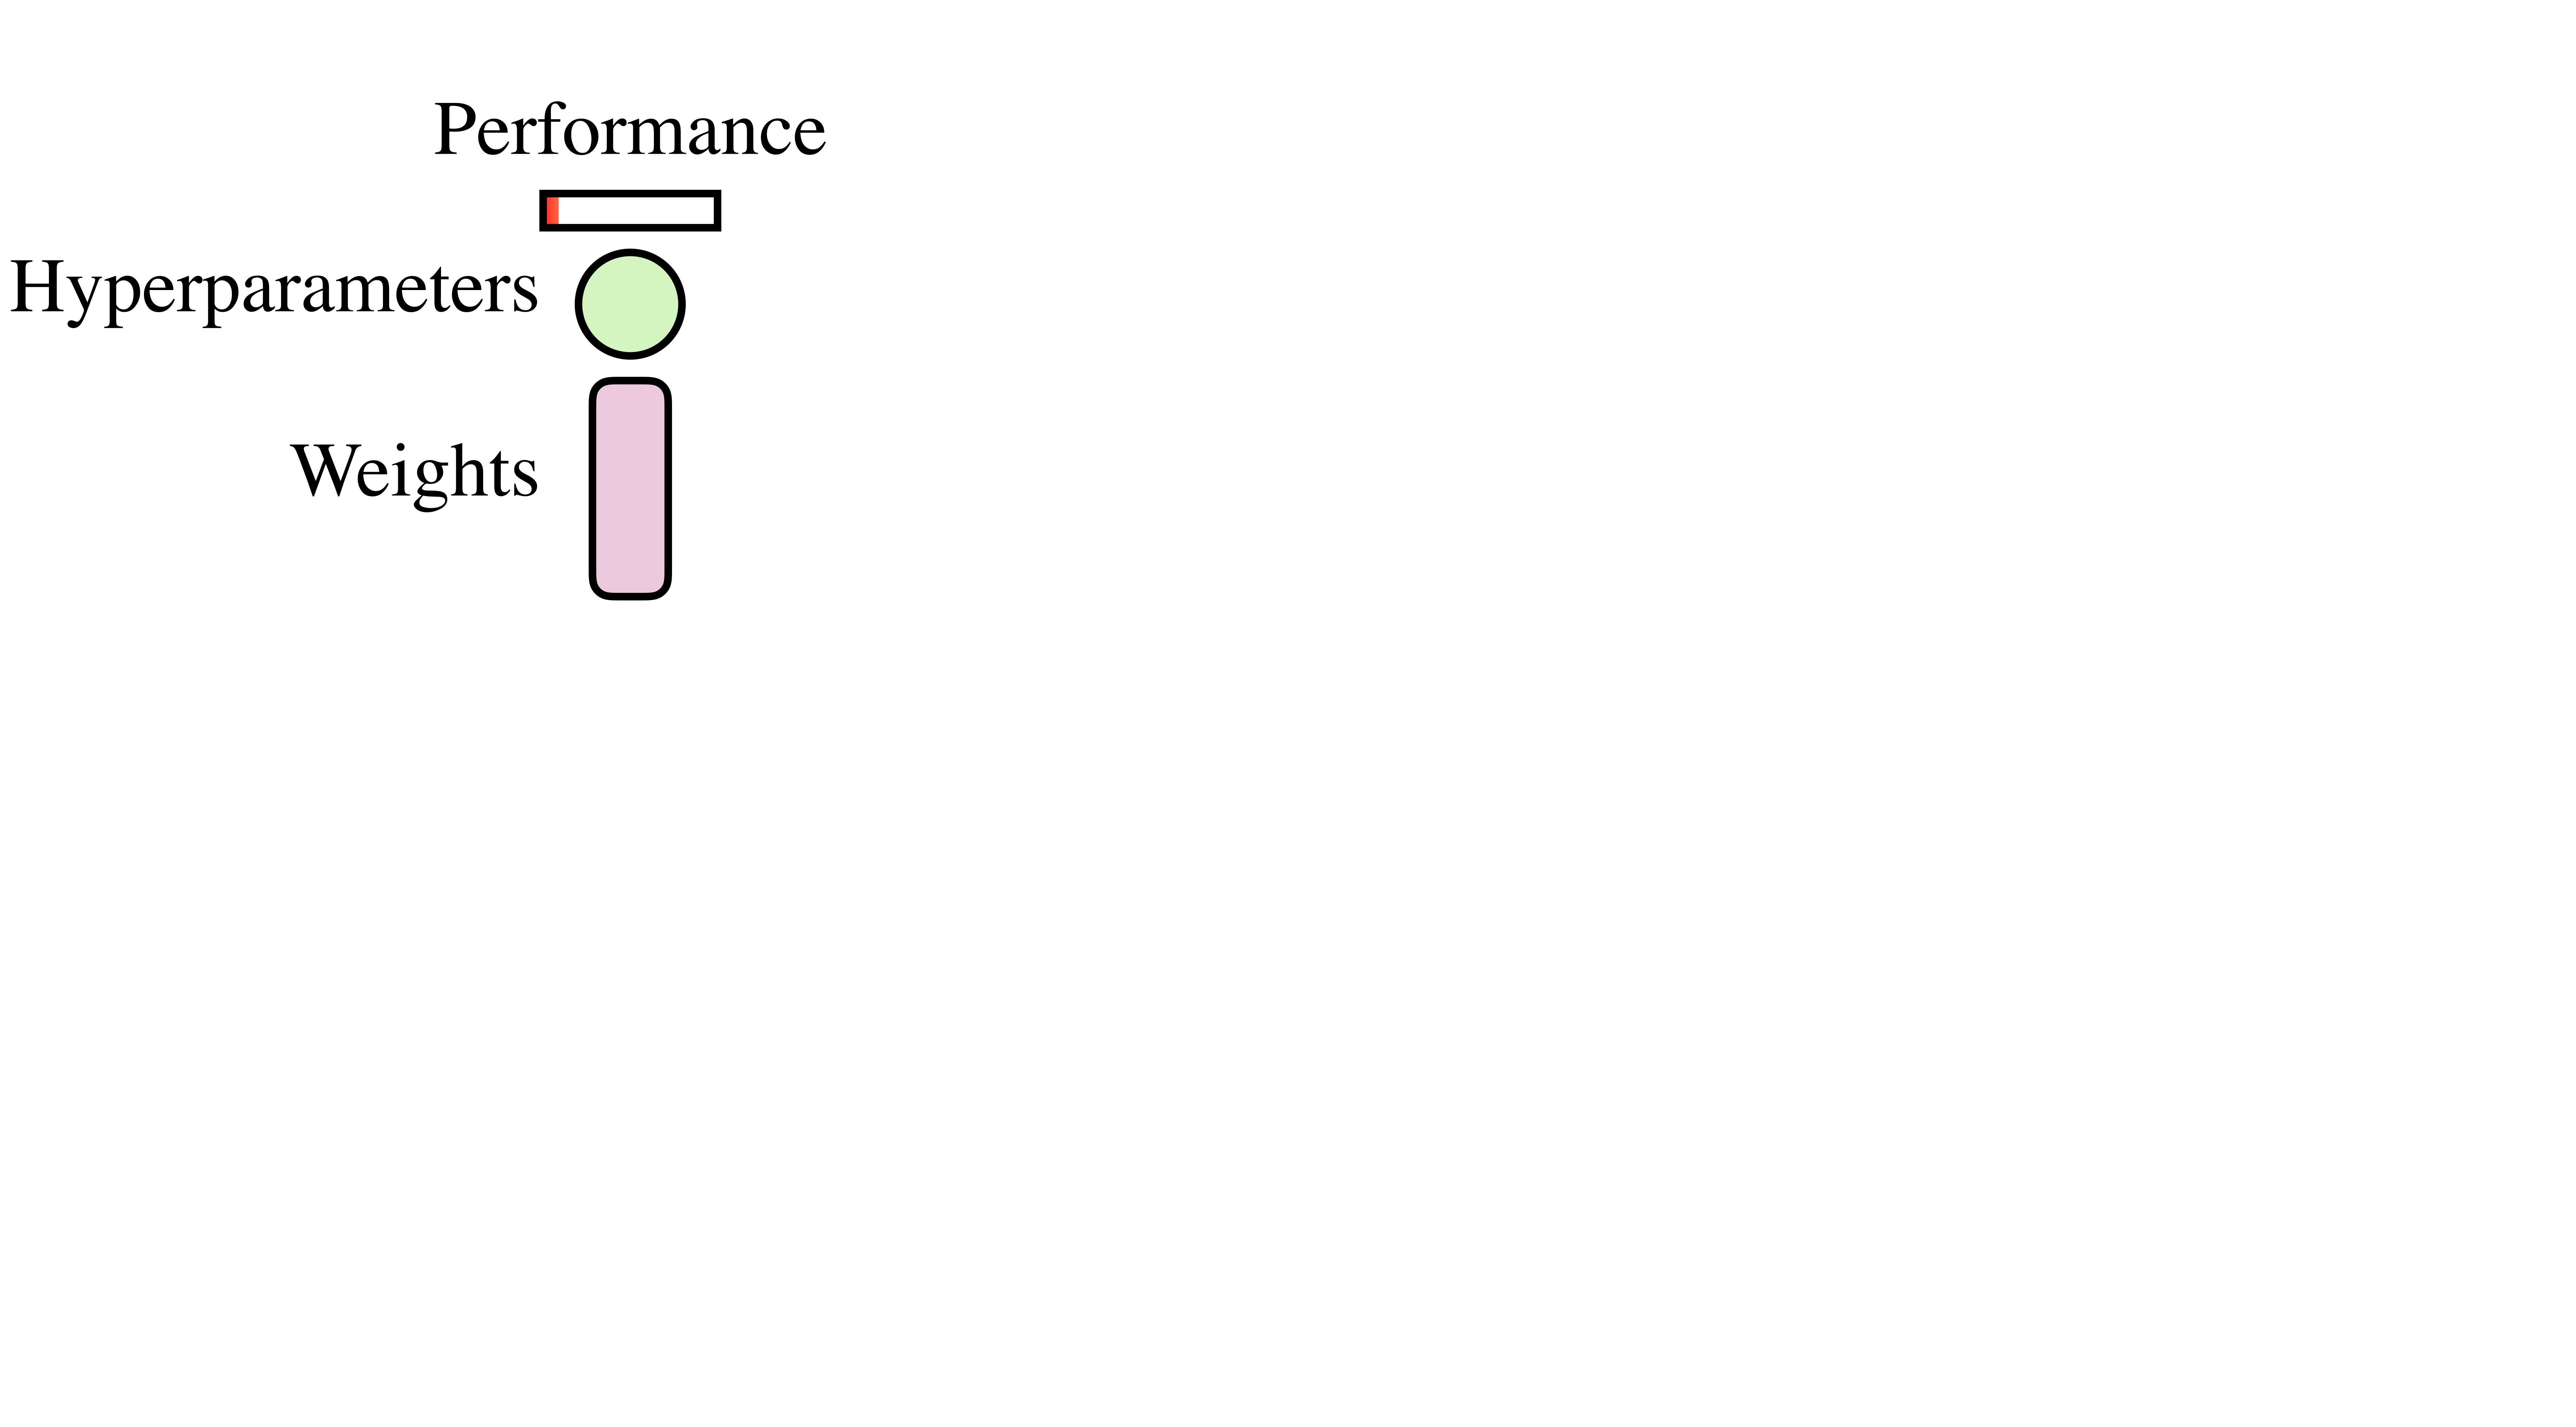
\includegraphics[width=.75\linewidth]{images/pbt_a}\\
        \liturl{Based on Figure 1 of Jaderberg et al. 2017}{https://arxiv.org/abs/1711.09846}
\end{frame}
%-----------------------------------------------------------------------
%----------------------------------------------------------------------
\begin{frame}{Sequential Training}
        \centering
        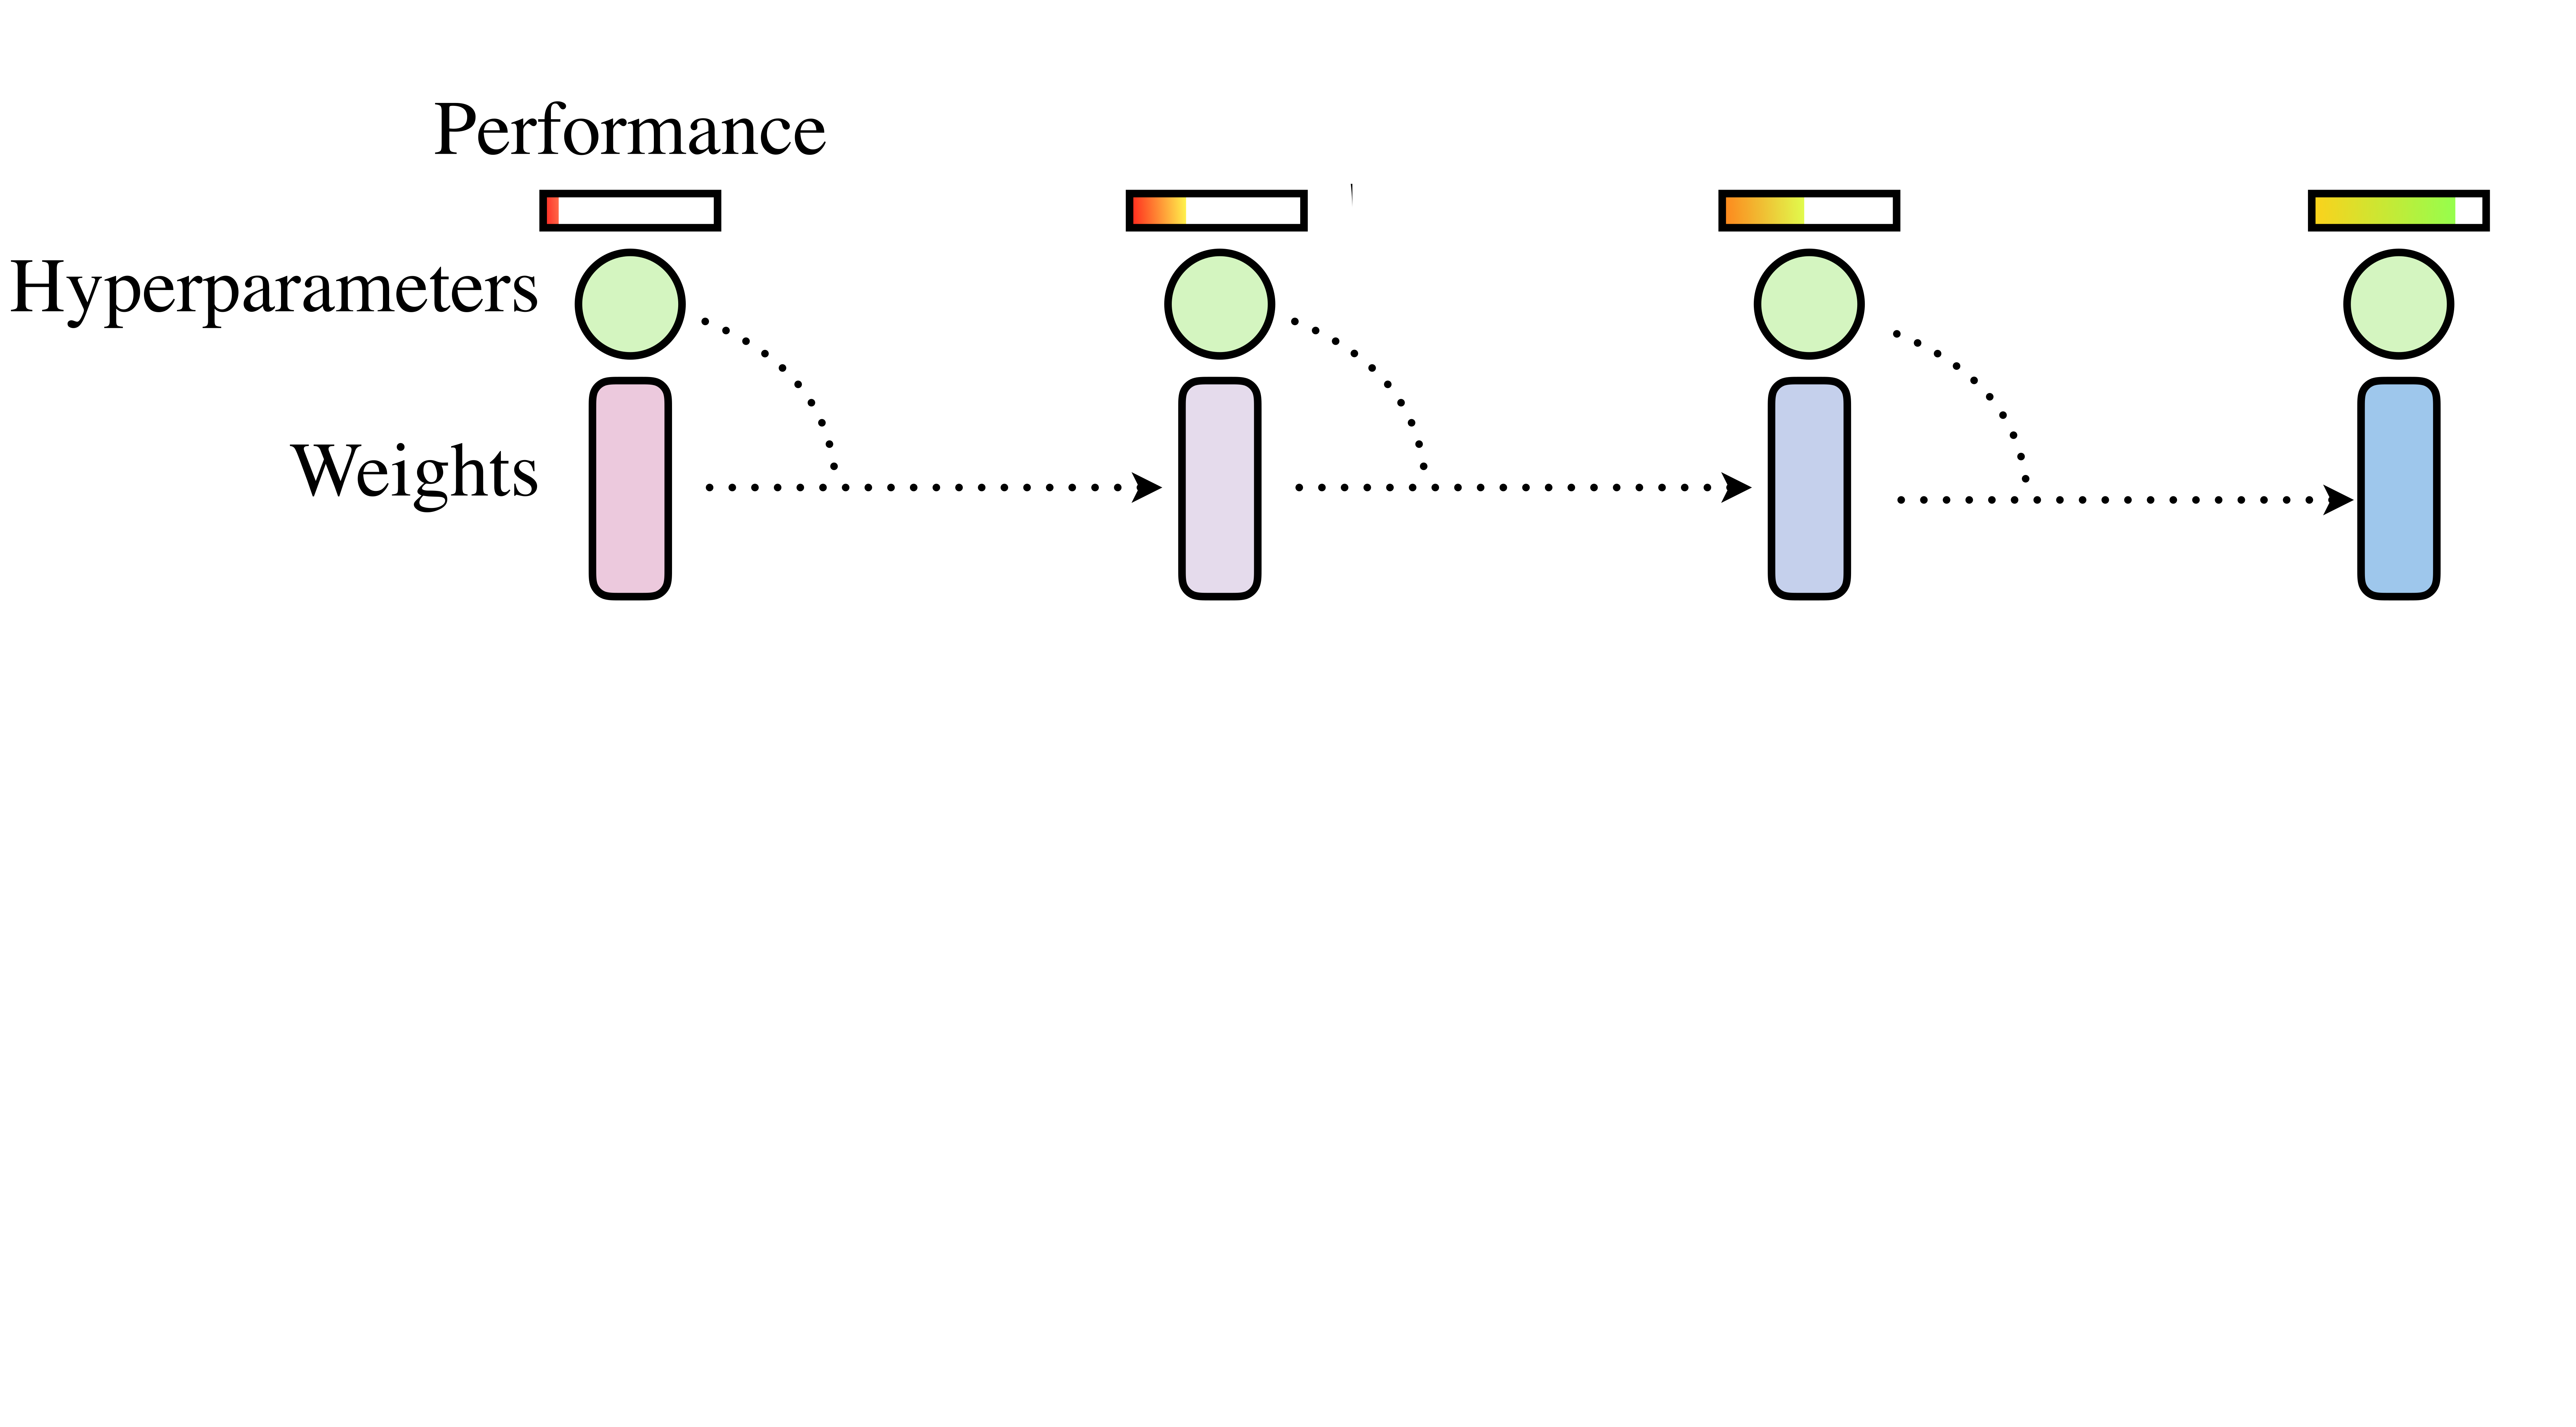
\includegraphics[width=.75\linewidth]{images/pbt_b}\\
        \liturl{Based on Figure 1 of Jaderberg et al. 2017}{https://arxiv.org/abs/1711.09846}
\end{frame}
%-----------------------------------------------------------------------
%----------------------------------------------------------------------
\begin{frame}{Parallel Training}
        \centering
        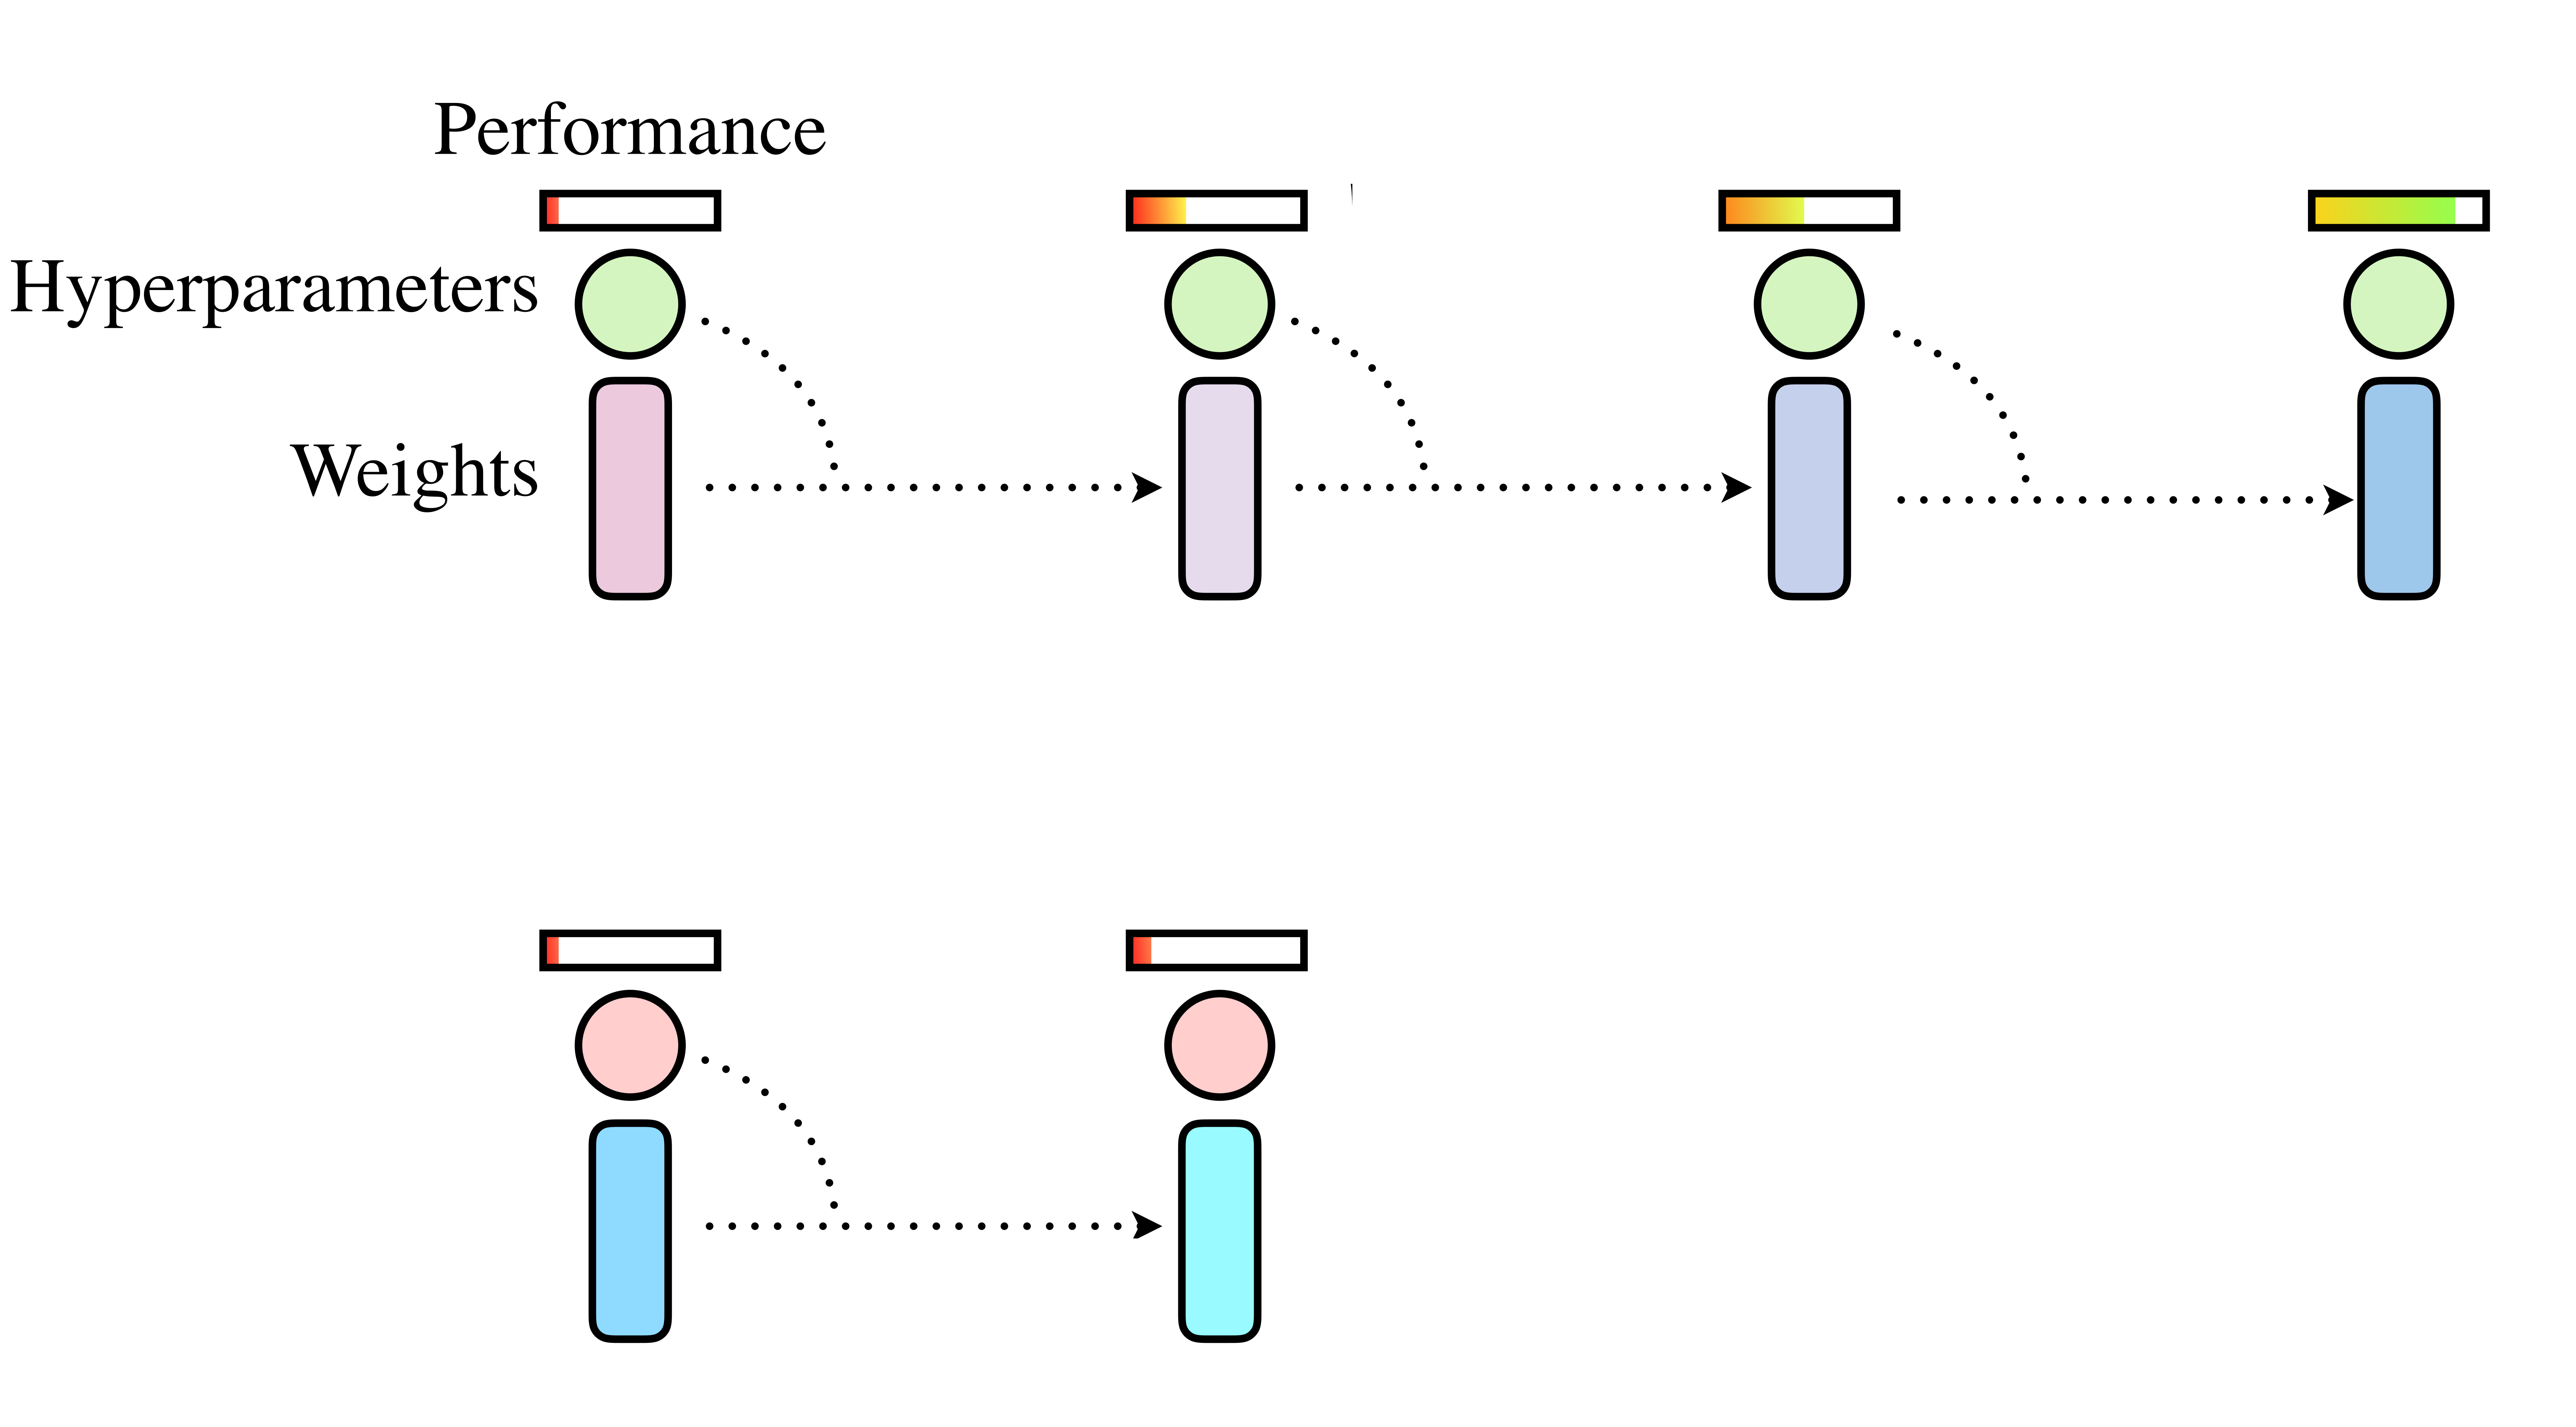
\includegraphics[width=.75\linewidth]{images/pbt_c}\\
        \liturl{Based on Figure 1 of Jaderberg et al. 2017}{https://arxiv.org/abs/1711.09846}
\end{frame}
%-----------------------------------------------------------------------
%----------------------------------------------------------------------
\begin{frame}{Population-Based Training (PBT) \liturl{Jaderberg et al. 2017}{https://arxiv.org/abs/1711.09846}}
        \centering
        \only<1>{
        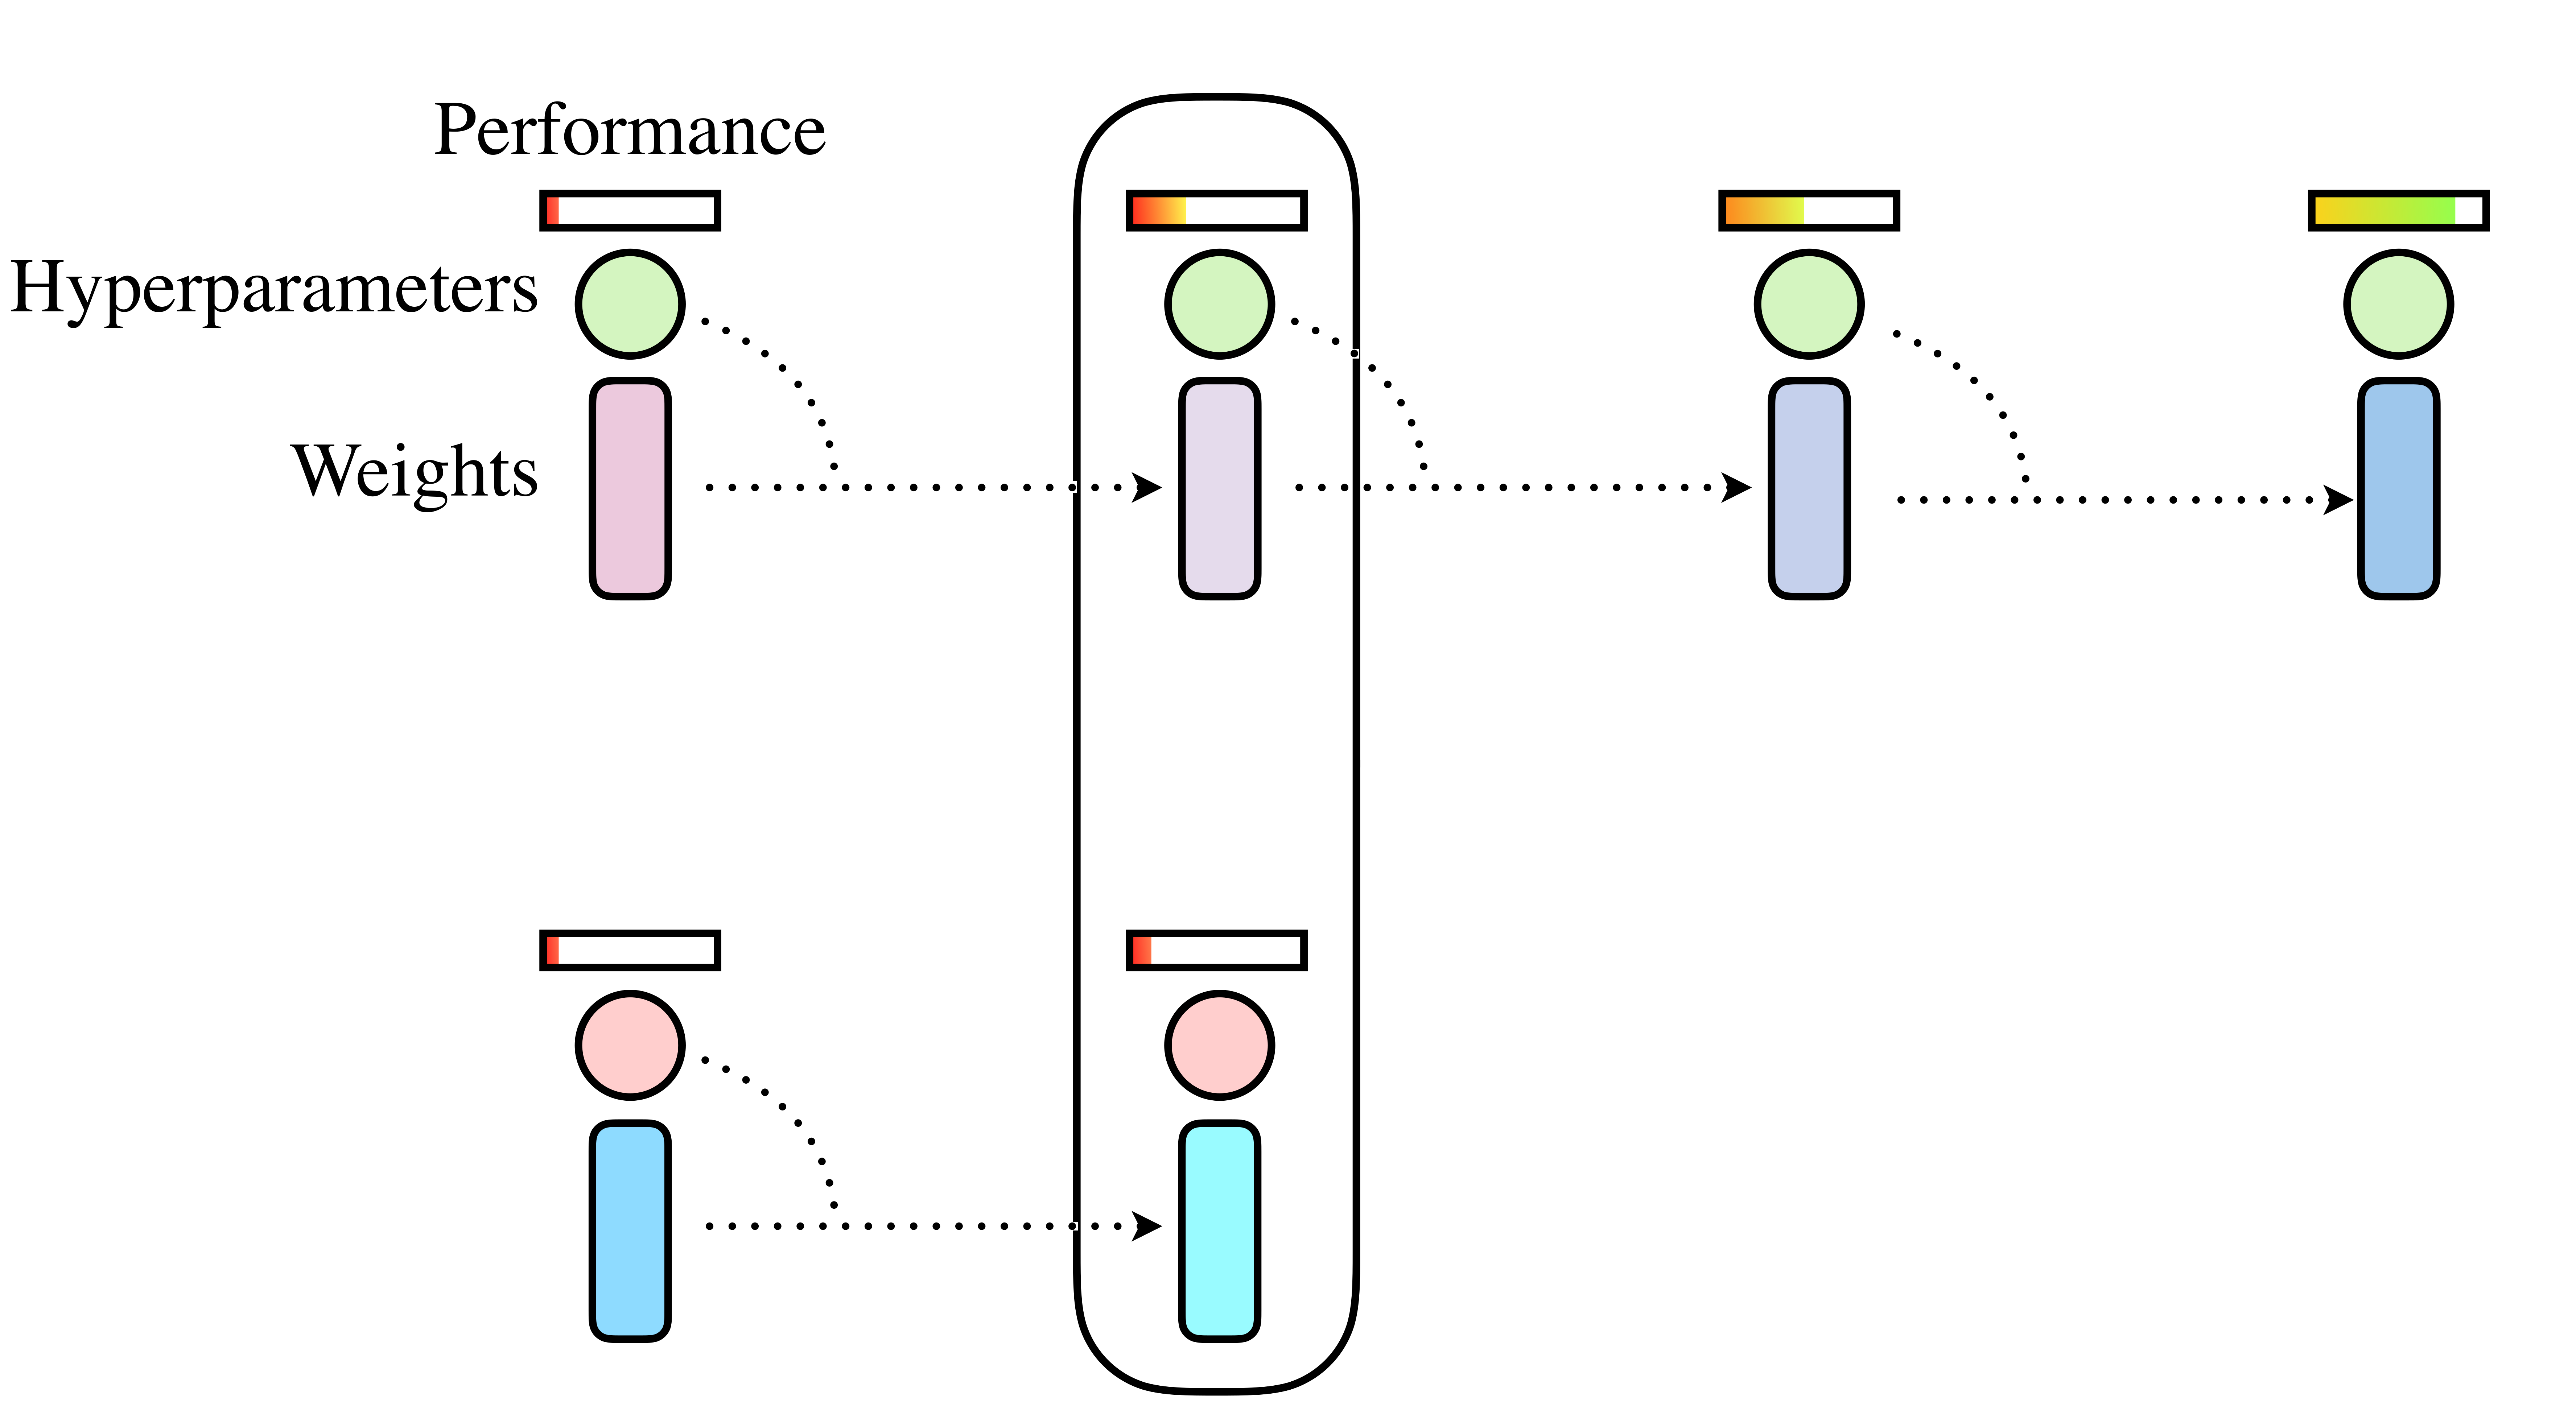
\includegraphics[width=.75\linewidth]{images/pbt_d}}
        \onslide<2->{
        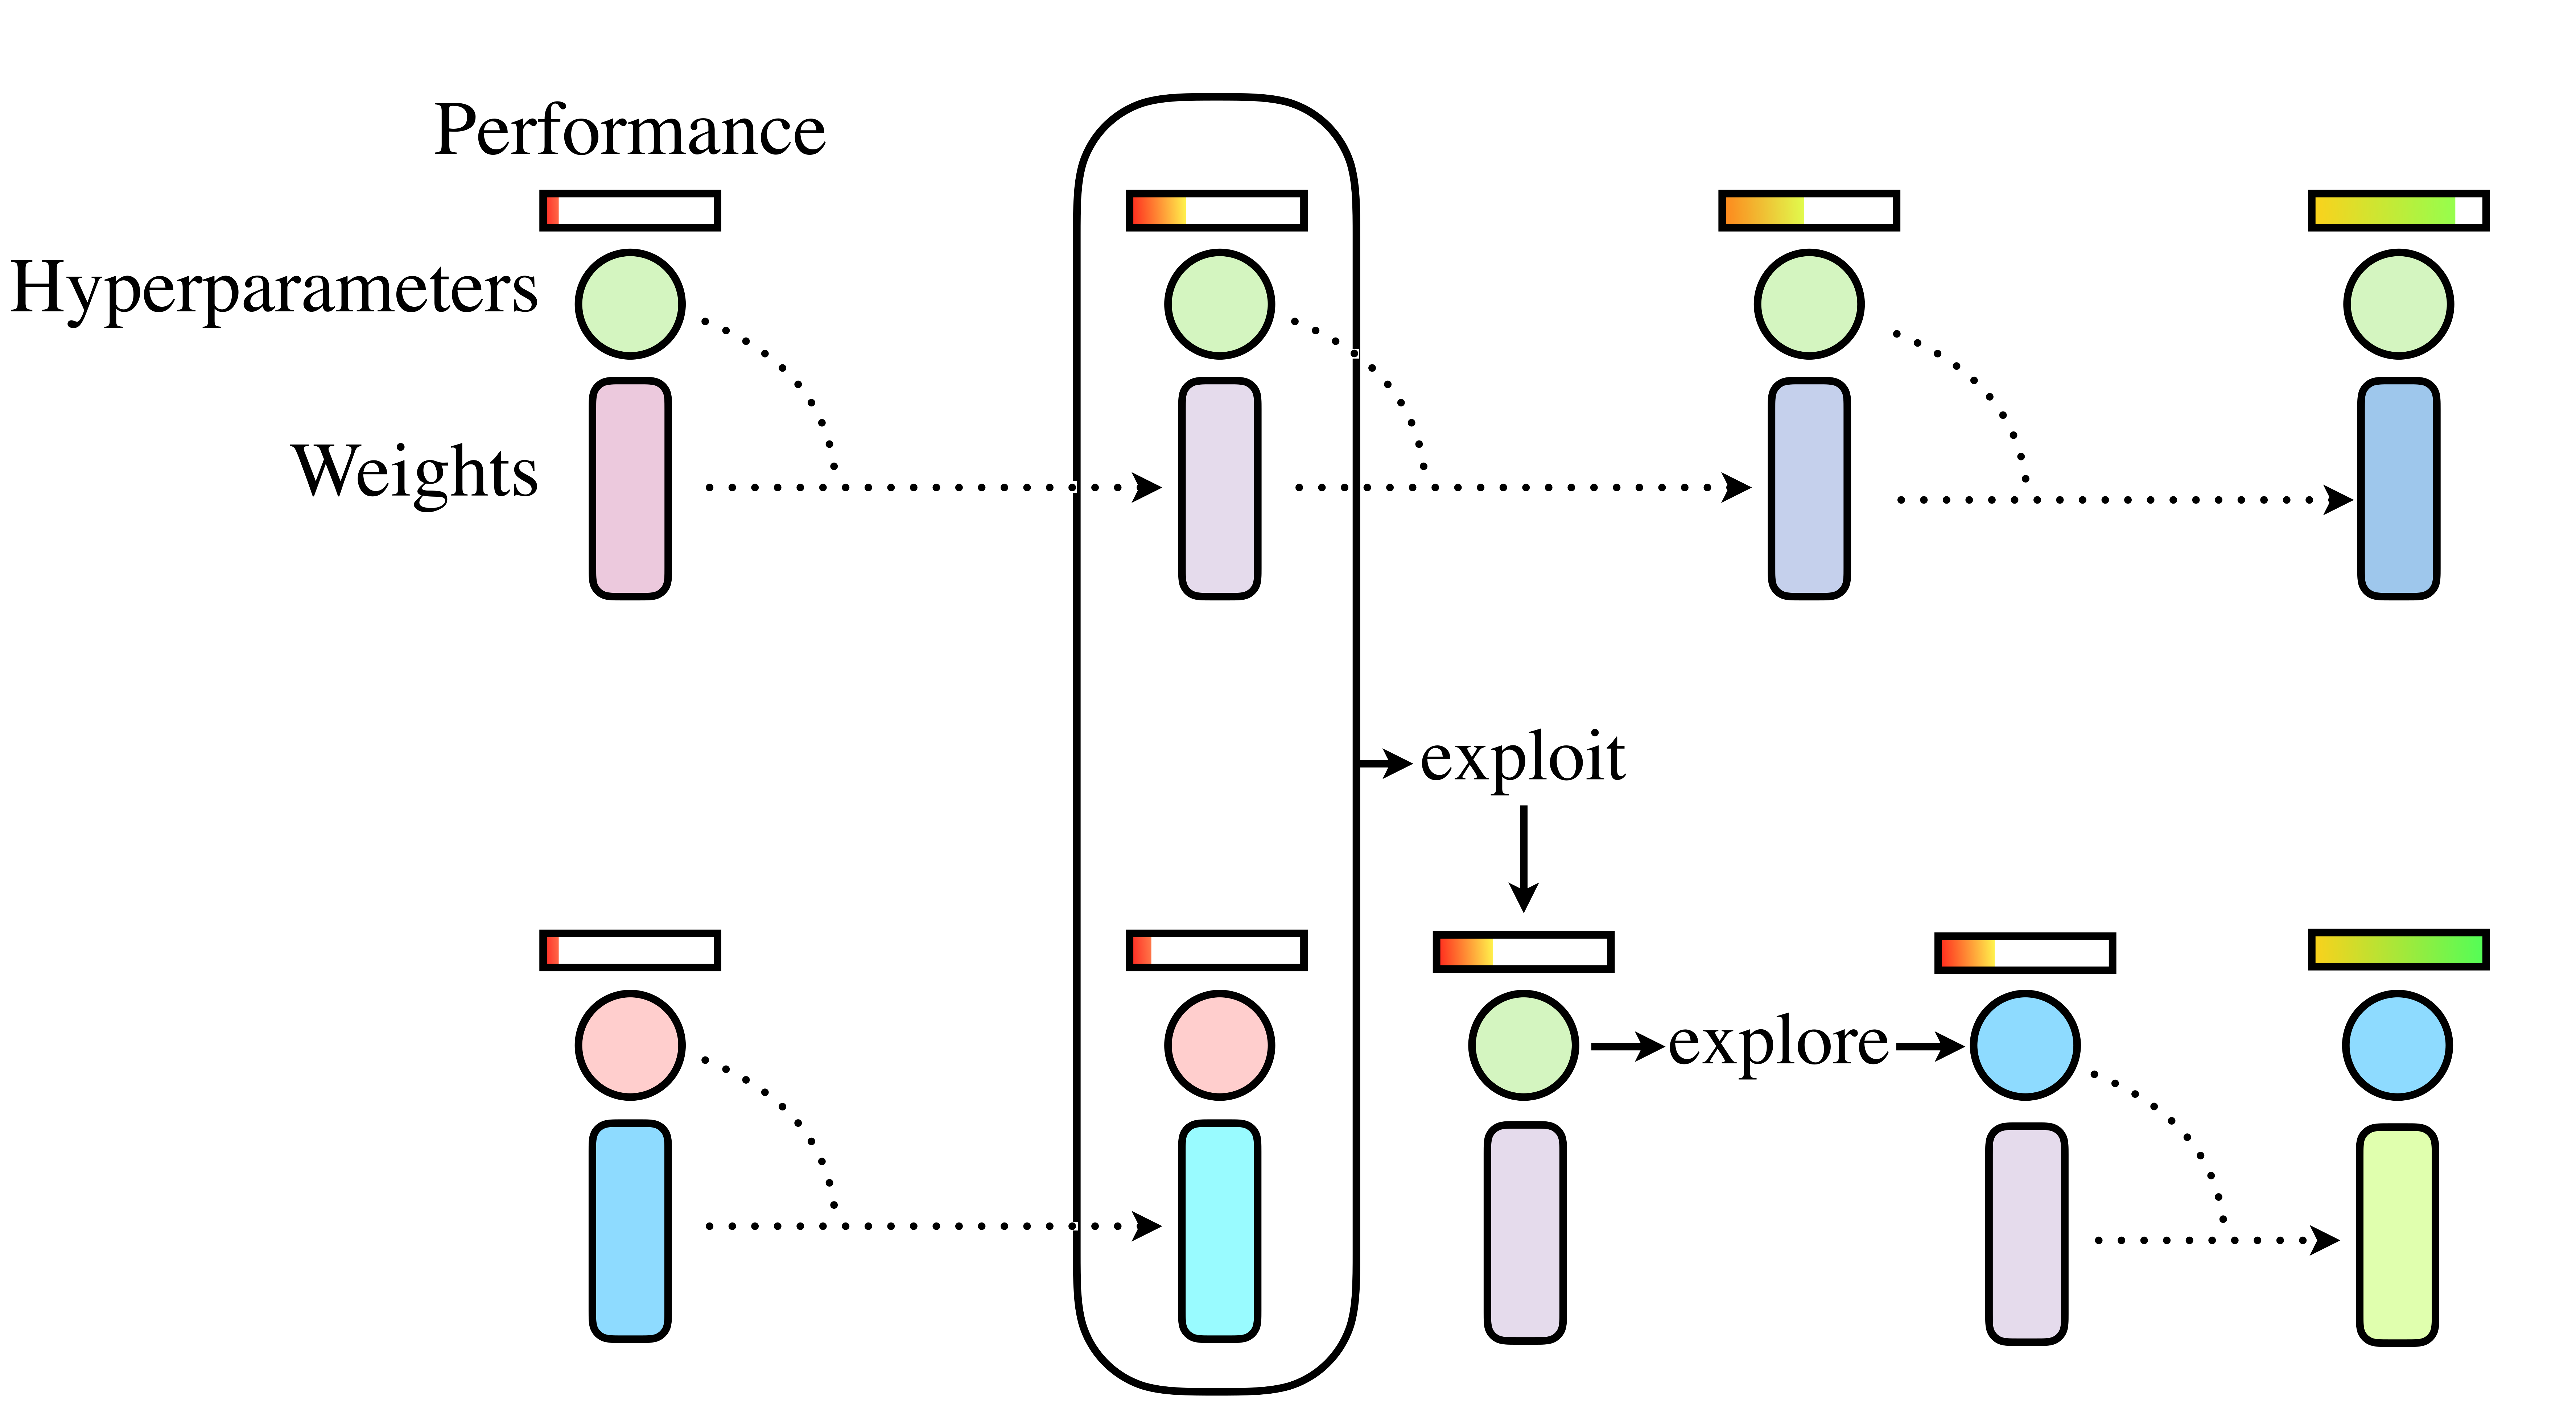
\includegraphics[width=.75\linewidth]{images/pbt_e}}\\\pause
        Exploit: Copy over well performing model weights -- Explore: Perturb Hyperparameters
\end{frame}
%-----------------------------------------------------------------------
%----------------------------------------------------------------------
\begin{frame}{Population-Based Training (PBT) - Example \liturl{Jaderberg et al. 2017}{https://arxiv.org/abs/1711.09846}}
        \centering
        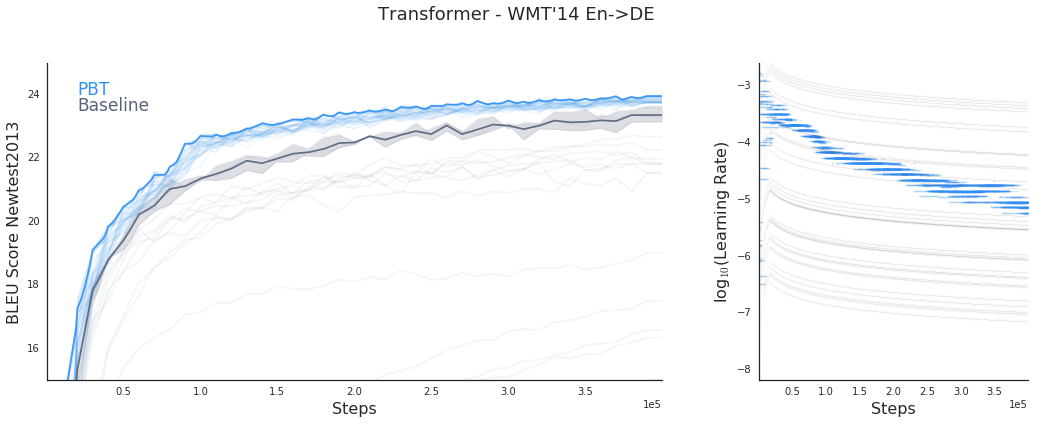
\includegraphics[width=\linewidth]{images/bigind_mt_lr_only}
\end{frame}
%-----------------------------------------------------------------------
%----------------------------------------------------------------------
\begin{frame}{Properties of PBT}
    \begin{itemize}
        \item PBT does \alert{not} return a hyperparameter optimization policy\pause
        \item PBT returns a fully trained model\pause
        \item PBT uses evolution to trade-off exploration and exploitation (not model based) of hyperparameter performance (see also \liturl{Elfwing et al. 2017}{https://arxiv.org/abs/1702.07490})\pause
        \item Efficiently parallelizable due to independent member training
    \end{itemize}
\end{frame}
%-----------------------------------------------------------------------
%----------------------------------------------------------------------
\begin{frame}{Combining PBT and Bayesian Optimization}
    \begin{itemize}
        \item Bayesian Optimization (BO) is well known for its sample efficiency\pause
        \item Can BO guide PBTs exploration?\pause
        \item Yes (\liturl{Parker-Holder et al. 2020}{https://proceedings.neurips.cc/paper/2020/hash/c7af0926b294e47e52e46cfebe173f20-Abstract.html},\liturl{Wan et al. 2022}{https://proceedings.mlr.press/v188/wan22a.html}), but ...
        \begin{itemize}
            \item PBT can run asynchronously $\leadsto$ force synchronicity or use approaches for parallel BO\pause
            \item Cost $\cost(\conf^{(t)})$ of the next configuraiton $\conf^{(t)}$ depends on $\conf^{(t-1)}, \conf^{(t-2)}, \ldots, \conf^{(1)}$
            \begin{itemize}
                \item Predict cost improvement $\surro(\conf^{(t)})=\frac{\cost(\conf^{(t-1)})-\cost(\conf^{(t-2)})}{\Delta t}$
                \item Add $\cost(\conf^{(t-1)})$ as input to the surrogate to ease the predicting the improvement
            \end{itemize}\pause
            \item PBT + BO introduced by Population Based Bandits (PB2 \liturl{Parker-Holder et al. 2020}{https://proceedings.neurips.cc/paper/2020/hash/c7af0926b294e47e52e46cfebe173f20-Abstract.html})
        \end{itemize}
    \end{itemize}
\end{frame}
%-----------------------------------------------------------------------
%----------------------------------------------------------------------
\begin{frame}{Bayesian Generational PBT \liturl{Wan et al. 2022}{https://proceedings.mlr.press/v188/wan22a.html}}
        \centering
        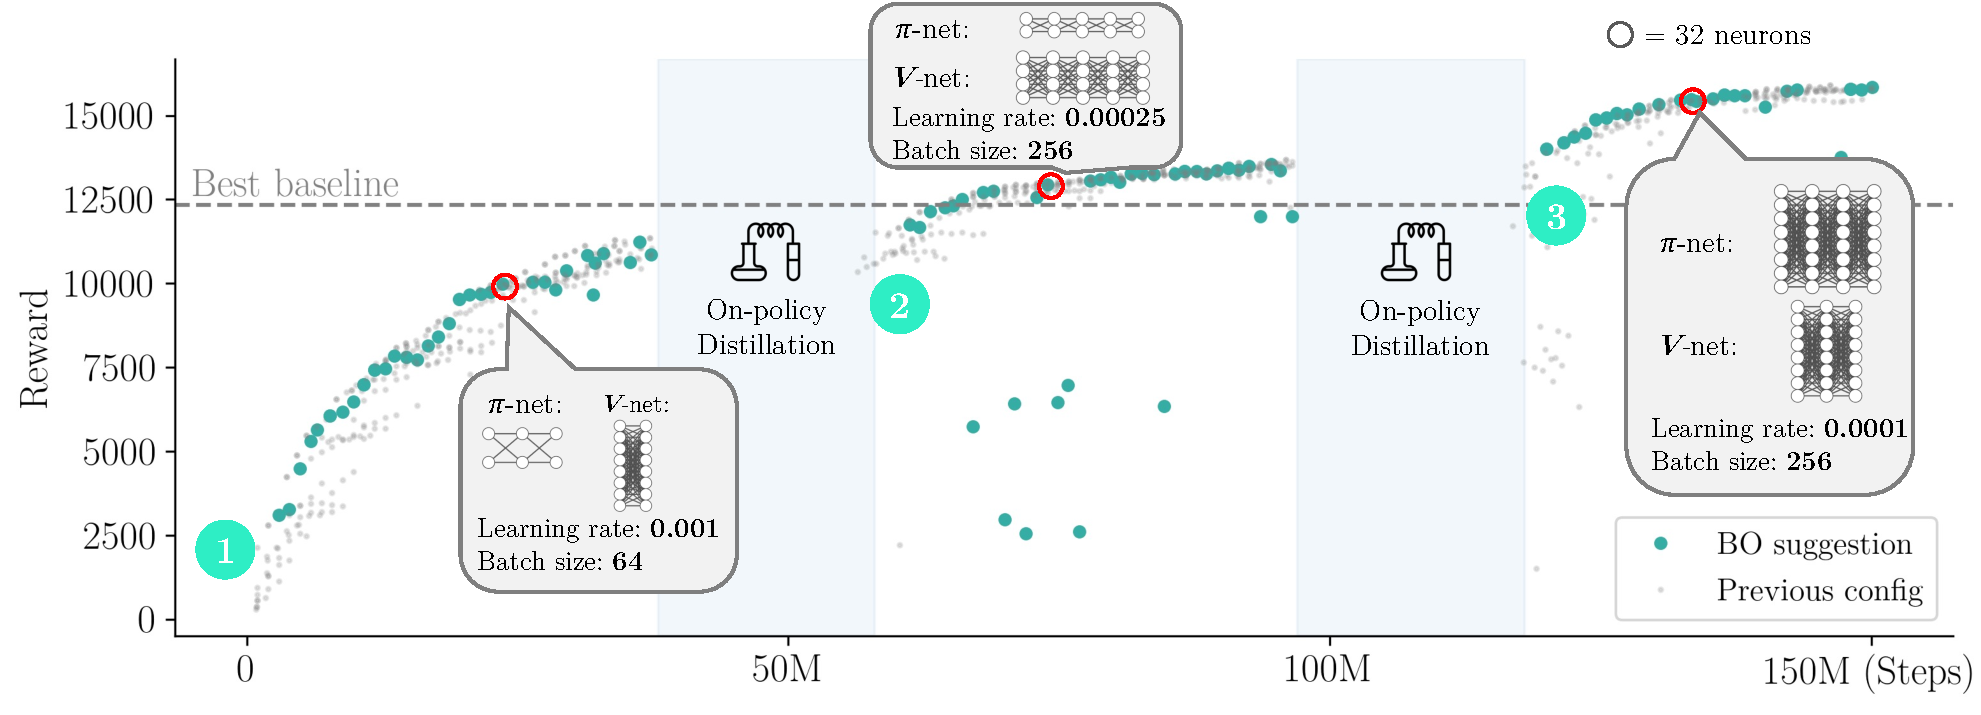
\includegraphics[width=\linewidth]{images/bgpbt.pdf}\\
        Incorporates NAS via architecture sampling and distillation
\end{frame}
%-----------------------------------------------------------------------
%----------------------------------------------------------------------
\begin{frame}{Meta Population Based Bandits \liturl{Hog et al. 2025}{https://openreview.net/forum?id=d9htascfP8}}
        \centering
        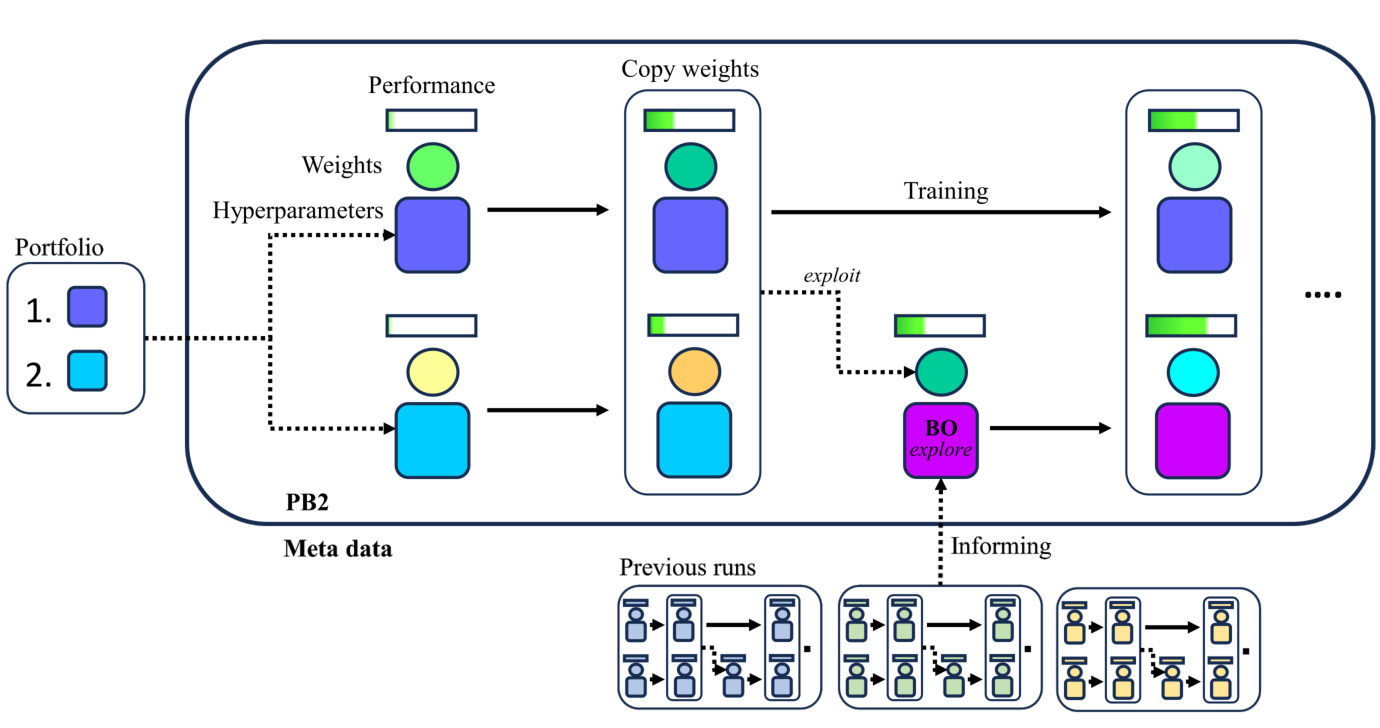
\includegraphics[width=.75\linewidth]{images/mpb2_overview.pdf}\\
        Enables implicit reuse of schedules via meta-learning
\end{frame}
%-----------------------------------------------------------------------
%----------------------------------------------------------------------
\begin{frame}{Main Takeaways} 

%Most important insights from this video:

\begin{itemize}
    \item \textbf{Dynamic tuning via evolution:} PBT and its variants explore hyperparameter schedules via changes in schedules for well-performing candidates.
    \item \textbf{Successors incorporate prior knowledge in various ways:} 
    \begin{itemize}
        \item PB2 builds a surrogate based on previous performance,
        \item BG-PBT uses distillation to transfer performance across architecture generations,
        \item Meta-PB2 uses meta-learning techniques for BO to incorporate more knowledge of prior tuning experiments.
    \end{itemize}
    \item \textbf{PBT-style HPO does \alert{not} produce (re-)usable schedules.}
\end{itemize}

\end{frame}


	

%----------------------------------------------------------------------
%----------------------------------------------------------------------
% \begin{frame}[c]{Planning Slide}
% \begin{enumerate}
%     \item PBT to connect with evolutionary Algorithms for HPO
%     \item PB2 to connect to BO and HPO BO
%     \item MetaPB2 to connect to ensembling?
%     \item Alternatively BG-PBT or SEARL to discuss dynamic network evolution??
%     \item Highlight shortcomings to motivate why learned methoods might be better
% \end{enumerate}
% \end{frame}
%-----------------------------------------------------------------------

\end{document}
